\documentclass[border=10pt]{standalone}
\usepackage{pgfplots}
\usetikzlibrary{calc, intersections, decorations.markings, decorations.pathmorphing, angles, quotes}
\colorlet{bgcolor}{red}
\begin{document}

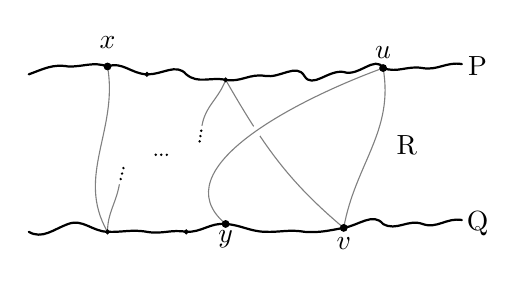
\begin{tikzpicture}[line cap=round]

%Coordinates	
\coordinate (P) at (0.5,2.1);
\coordinate (Q) at (0.5,0.1);

\coordinate (R) at (-0.2,1);
\coordinate (etc3) at (-3.3,1);


%  Path P
\draw[thick]
	(-5,2) to[out=20, in=170] ++(0.5,0.1)
		   to[out=-2, in=160] ++(0.5,+0) coordinate (x)
		   to[out=+20, in=178] ++(0.5,-0.1)  coordinate (top1)
		   to[out=-2, in=130] ++(0.5,+0)
		   to[out=-40, in=168] ++(0.5,-0.07)		coordinate (top2)  
		   to[out=-10, in=170] ++(0.5,+0.05) 	   
		   to[out=-10, in=120] ++(0.5,0) 
		   to[out=300, in=170] ++(0.5,+0.05) 	   
		   to[out=-20, in=120] ++(0.5,+0.05) coordinate (u)	   
		   to[out=-20, in=170] ++(0.5,0) 
		   to[out=-10, in=170] ++(0.5,+0.05) 	   
	;

% Path Q

\draw[thick]
	(-5,0) to[out=-30, in=-160] ++(0.5,0.1)
		   to[out=20, in=178] ++(0.5,-0.1) coordinate (bottom1)
		   to[out=-2, in=170] ++(0.5,+0)
		   to[out=-10, in=170] ++(0.5,0)  coordinate (bottom2)
		   to[out=-2, in=175] ++(0.5,+0.1) coordinate (y)
		   to[out=-4, in=178] ++(0.5,-0.1) 
	 	   to[out=-2, in=170] ++(0.5,+0) 
		   to[out=-4, in=190] ++(0.5,0.05) coordinate (v)
		   to[out=+10, in=130] ++(0.5,+0.05) 	   
		   to[out=-30, in=160] ++(0.5,0) 
		   to[out=-20, in=170] ++(0.5,+0.05) 
	;

%1st dots

\coordinate (end1) at ($(bottom1)!0.3!(top1)$);
\coordinate (etc1) at ($(end1)!0.1!(top1)$);


\draw[fill=black, draw=black]  ($(end1)!0.5!(etc1)$) circle (0.2pt);
\draw[fill=black, draw=black]  (etc1) circle (0.2pt);
\draw[fill=black, draw=black]  ($(end1)!1.5!(etc1)$) circle (0.2pt);
	
	
%% middle dots
	


% 3rd dots


\coordinate (end2) at ( $(bottom2)!0.7!(top2) - (0.15,0)$ );
\coordinate (etc2) at ($(end2)!0.1!(bottom2)$);


\draw[fill=black, draw=black]  ($(end2)!0.5!(etc2)$) circle (0.2pt);
\draw[fill=black, draw=black]  (etc2) circle (0.2pt);
\draw[fill=black, draw=black]  ($(end2)!1.5!(etc2)$) circle (0.2pt);


\coordinate (middle) at ($(etc1)!0.5!(etc2)$-,1);


\draw[fill=black, draw=black]  ($(middle)-(0.07,0)$) circle (0.2pt);
\draw[fill=black, draw=black]  (middle) circle (0.2pt);
\draw[fill=black, draw=black]  ($(middle)+(0.07,0)$) circle (0.2pt);


%%%%%%%%%%%% 
% Paths

\draw[gray] (x) to[out=280, in=120] (bottom1); 
%
%not finishing paths
	\draw[gray] (bottom1) to[out=90, in=260] (end1);
	\draw[gray] (top2) to[out=250, in=80] (end2);
%
\draw[gray] (top2) to[out=300, in=140] (v);
\draw[gray] (v) to[out=80, in=280] (u); 
% to make hover effect
\draw[white, line width=4pt] ($(u)+(-0.5,-0.21) $)  to[out=200, in=140] ($(y)+(0.15,0.3)$);
\draw[gray, name path = uy] (u) to[out=200, in=140] (y); 

% Nodes
\node[shift={(0.2,0)}] at (P) {$\mathrm{P}$};
\node[shift={(0.2,0)}] at (Q) {$\mathrm{Q}$};
\node[shift={(0,0.1)}] at (R) {$\mathrm{R}$};
\node[shift={(0,0.3)}] at (x) {$x$};
\node[shift={(0,0.2)}] at (u) {$u$};
\node[shift={(0,-0.2)}] at (y) {$y$};
\node[shift={(0,-0.2)}] at (v) {$v$};


% Small Points
\draw[fill=black, draw=black] (top1) circle (0.7pt);
\draw[fill=black, draw=black] (top2) circle (0.7pt);
\draw[fill=black, draw=black] (bottom1) circle (0.7pt);
\draw[fill=black, draw=black] (bottom2) circle (0.7pt);

% Points

\draw[fill=black, draw=black] (x) circle (1.2pt);
\draw[fill=black, draw=black] (y) circle (1.2pt);
\draw[fill=black, draw=black] (u) circle (1.2pt);
\draw[fill=black, draw=black] (v) circle (1.2pt);




\end{tikzpicture}
\end{document}